\documentclass[10pt,a4paper]{article}
\usepackage[T1]{fontenc}
\usepackage[utf8]{inputenc}
\usepackage{mathpazo}
\usepackage[scaled=0.9]{helvet}
\usepackage{courier}
\usepackage[margin=2.3cm]{geometry}
\usepackage{microtype}
\usepackage{booktabs}
\usepackage{array}
\newcolumntype{L}[1]{>{\raggedright\arraybackslash}p{#1}}
\usepackage{siunitx}
\usepackage{xcolor}
\usepackage{enumitem}
\usepackage{caption}
\usepackage{pgfplots}
\pgfplotsset{compat=1.17}
\usepackage{tcolorbox}
\usepackage{fancyhdr}
\usepackage{titlesec}
\usepackage[colorlinks=true,linkcolor=skyink,urlcolor=skyink,citecolor=skyink]{hyperref}

\definecolor{sky}{HTML}{3FA9F5}
\definecolor{skyink}{HTML}{1F6FB0}
\definecolor{ffyellow}{HTML}{F3D630}
\definecolor{ink}{HTML}{1A1A1A}
\definecolor{protoc}{HTML}{3FA9F5}
\definecolor{capnpc}{HTML}{C9A400}
\definecolor{greyc}{HTML}{9A9A9A}

\sisetup{group-separator={\,},group-minimum-digits=4,detect-all}
\setlist{itemsep=2pt,topsep=4pt}
\titleformat{\section}{\large\sffamily\bfseries\color{ink}}{\thesection}{0.8em}{}[{\color{sky}\titlerule[0.8pt]}]
\titleformat{\subsection}{\normalsize\sffamily\bfseries\color{ink}}{\thesubsection}{0.8em}{}
\pagestyle{fancy}\fancyhf{}
\renewcommand{\headrulewidth}{0pt}
\fancyfoot[L]{\sffamily\footnotesize F1R3FLY.io --- research note}
\fancyfoot[R]{\sffamily\footnotesize\thepage}

\makeatletter\g@addto@macro{\UrlBreaks}{\do\_\do\.\do\(\do\:\do\-}\makeatother
\urlstyle{tt}
\newcommand{\f}[1]{\nolinkurl{#1}}
\newcommand{\capnp}{Cap'n~Proto}
\newtcolorbox{finding}[1][]{colback=sky!6,colframe=sky,boxrule=0.6pt,arc=1pt,left=6pt,right=6pt,top=4pt,bottom=4pt,fonttitle=\sffamily\bfseries\small,#1}

\title{\sffamily\bfseries Protobuf to \capnp{} in \f{f1r3node-rust}:\\[2pt]
\large\mdseries where the performance is, and what a port would cost}
\author{\sffamily F1R3FLY.io}
\date{\sffamily 20 October 2026 (revised) \quad$\cdot$\quad \f{dev} @ \f{e87572d}}

\emergencystretch=3em
\begin{document}
\maketitle
\thispagestyle{fancy}

\begin{abstract}
\noindent This note asks whether replacing Protocol Buffers (prost/tonic) with \capnp{} in
\f{f1r3node-rust} would yield worthwhile performance gains, and what such a port would cost.
\f{f1r3node-rust} is a platform: organisations stand up their own shards with it, from the
Artificial Superintelligence Alliance's ASI:Chain to internal deployments, and shards are cheap to
create. An encoding change is therefore a \emph{shard-format release} that each deployment adopts
on its own schedule, not a fork of one shared history. The answer has three parts. First, the
protobuf encoding is more than a wire format: it is the input to the block hash, deploy signatures,
unforgeable-name seeds, registry signatures, address derivation and Rholang's \f{toByteArray}. A
port has to choose a canonical hashing encoding for all of these and update every client SDK's
deploy signing. Second, micro\-benchmarks on the node's own message shapes show \capnp{} encodes
1.4--2.4$\times$ faster (except for small terms) and reads in place 3--5$\times$ faster, but
materialising owned Rust structures from \capnp{} is \emph{slower} than prost (1.1--2$\times$), its
canonical form for hashing is 3.6--7$\times$ slower, and unpacked messages are 43\% (blocks) to
nearly 7$\times$ (Rholang terms) larger. Third, the whole protobuf codec bill for a typical
32-deploy block is about 1\,ms per validator, against roughly 320\,ms of deploy evaluation; the
best realistic \capnp{} port recovers about 0.5\,ms of it. The recommendation is not to port,
because the gain is too small for the work. The prost-side fixes in Section~\ref{sec:recs}
recover more for a few lines of code. Since hash formats can be changed per release, a Merkle-root
block hash is the better use of that freedom: it takes the end-of-block hash check from
463 to 7\,\si{\micro\second} and gives per-deploy inclusion proofs. Serialisation effort beyond
that belongs on RSpace's bincode hashing, which runs on every produce and consume.
\end{abstract}

\section{Scope and method}

The analysis covers the \f{dev} branch of \f{F1R3FLY-io/f1r3node-rust} at commit \f{e87572d}
(merge of PR \#662, 20~October~2026). It has three parts.
\begin{enumerate}
  \item An inventory of every protobuf schema and every encode/decode call site, classified by the
        role the bytes play (wire, storage, hash input, in-memory type, external API).
  \item A standalone benchmark crate that compiles the repository's real \f{CasperMessage.proto} and
        \f{RhoTypes.proto} with the same prost-build settings the node uses (\f{btree_map(".")},
        \f{Bytes} for \f{.casper}/\f{.routing}), alongside a \capnp{} schema mirroring the same
        fields. Round-trip equality is asserted for every workload before timing.
  \item A per-block budget combining the benchmark numbers with the call paths found in (1) and
        the node's own propose-latency measurements.
\end{enumerate}
\paragraph{Deployment context.} The node is software that other organisations run, each as one or
more shards: ASI:Chain is one such deployment and several companies run internal ones. Shards are
inexpensive to stand up and are separated by \f{networkId}. A change to a hashed or signed encoding
is therefore a new shard format shipped in a release. Existing shards keep running the release
they are on until their operators move; new shards start on the new format. The costs that remain
are engineering and ecosystem costs (client SDKs, tooling, contracts that depend on byte formats),
which this note estimates, rather than the preservation of a single history.

\medskip\noindent The node itself was not built: its pinned \f{nightly-2026-02-09} toolchain could not be fetched in
the analysis environment. Section~\ref{sec:validity} lists the consequences.

\section{Where protobuf lives in the node}

The repository carries 13 schema files (\num{2022} lines, 214 messages, 30 RPCs). Generated code
comes from \f{tonic-prost-build} in \f{models}, \f{comm} and \f{node}. Table~\ref{tab:roles}
groups the uses by the role of the bytes.

\begin{table}[h]
\centering\small
\begin{tabular}{@{}L{2.6cm}L{7.4cm}L{5.4cm}@{}}
\toprule
Role & What & Where (representative) \\
\midrule
P2P wire &
  \f{TransportLayer} gRPC (unary \f{Send}, client-streaming \f{Stream}); \f{Protocol}$\to$\texttt{Packet\{typeId, content\}} with the Casper message encoded inside (double encoding); 256\,KiB chunks; LZ4 above 500\,KB; rustls with node-id from cert. &
  \f{routing.proto:62}, \f{packet_type_tag.rs:29}, \f{chunker.rs:15}, \f{casper/src/rust/protocol/mod.rs:273} \\
Block storage &
  LMDB (heed). \f{blocks}: LZ4(prost(\f{BlockMessageProto})); \f{blocks-approved}: prost; deploy buffers: tagged prost. DAG indices, latest messages, casper buffer, finality: bincode. &
  \f{key_value_block_store.rs:263}, \f{deploy_codec.rs:24}, \f{block_dag_key_value_storage.rs:974} \\
Hash and signature input &
  Block hash, deploy signature, genesis approval, unforgeable seeds, registry signatures, \f{toByteArray}, unforgeable-to-address (Sec.~\ref{sec:consensus}). &
  \f{proto_util.rs:467}, \f{signed.rs:33}, \f{mergeable_tags.rs:55} \\
In-memory types &
  The generated \f{rhoapi} structs (\f{Par}, \f{Send}, \f{Expr}, \ldots) \emph{are} the interpreter's AST, with serde, \f{Ord} and utoipa derives added in \f{build.rs}. 542 import sites; 146 files in \f{rholang}, 63 in \f{casper}. &
  \f{models/build.rs:43-54} \\
External API &
  gRPC on 40401/40402: Deploy (19 RPCs), Propose, Repl, LSP, plus tonic-reflection; HTTP/JSON on 40403 via serde on the \f{rhoapi} types; clients include pyf1r3fly, system-integration, Embers, grpcurl. &
  \f{grpc_package.rs:117}, \f{web_api_routes.rs:40} \\
\bottomrule
\end{tabular}
\caption{Roles of protobuf bytes and types in \f{f1r3node-rust} (\f{dev}). Paths abbreviated.}
\label{tab:roles}
\end{table}

\noindent The serialiser that does the most work during block execution is not protobuf. RSpace
hashes every channel, datum and continuation by \f{bincode::serialize} followed by Blake2b256
(\f{stable_hash_provider.rs:7}), and trie leaves are bincode too
(\f{history_repository_impl.rs:226-330}). That path runs on every produce and consume.

\subsection{Encodings that feed hashes and signatures}\label{sec:consensus}

Each of the following hashes or signs prost output. Within a shard, every node must produce the
same bytes, so each of these is part of the shard format.

\begin{enumerate}
  \item \textbf{Block hash.} \f{hash_block} concatenates prost(\f{Header}), prost(\f{Body}) and
        raw fields, then Blake2b256 (\f{casper/src/rust/util/proto_util.rs:467-484});
        re-checked on every received block (\f{validate.rs:1179}).
  \item \textbf{Deploy signatures.} Wallets and clients sign Blake2b256 (or Keccak256 for
        eth-style keys) of prost(\f{DeployDataProto}) with \f{sig}/\f{deployer} cleared
        (\f{crypto/src/rust/signatures/signed.rs:33}; \f{casper_message.rs:1383}).
  \item \textbf{Genesis ceremony.} Approvals sign Blake2b256 of prost(\f{ApprovedBlockCandidate})
        (\f{validate.rs:167}); genesis deploy-log order is sorted by prost bytes
        (\f{genesis.rs:249}).
  \item \textbf{Unforgeable names.} The mergeable-tag RNG is seeded from
        prost(\texttt{DeployDataProto\{deployer, timestamp\}})
        (\f{rholang/.../merging/mergeable_tags.rs:49-56}).
  \item \textbf{Addresses and registry.} Unforgeable-to-address is Keccak256(prost(\f{GPrivate}))
        (\f{address_tools.rs:82}); registry signatures are Blake2b256(prost(\f{Par}))
        and are baked into the genesis contracts a shard ships with (\f{registry_sig_gen.rs:214}).
  \item \textbf{Language semantics.} Rholang's \f{toByteArray} returns prost(\f{Par})
        (\f{reduce.rs:3181}); contracts can store or hash the result.
\end{enumerate}

\begin{finding}[title=Consequence]
A port can replace prost entirely in a new shard format, so no permanent dual codec is forced. It
must still (i) pick one \emph{canonical} byte form for each of these six families, (ii) ship new
deploy-signing code in every client SDK (pyf1r3fly, Embers, partner wallets), (iii) regenerate the
signed genesis contracts, and (iv) document that \f{toByteArray} returns different bytes on the new
format. Section~\ref{sec:benchmarks} shows \capnp{} is a poor choice for (i), so a realistic port uses
\capnp{} on the wire and in storage and keeps a separate, simpler hashing encoding.
\end{finding}

\section{Benchmarks}\label{sec:benchmarks}

\subsection{Setup}
Workloads come from deterministic generators. Blocks follow \f{BlockMessageProto}: 5 validators
(bonds, justifications), 3 parents, and $N$ processed deploys, each carrying a 1.1\,KB Rholang
transfer term, 65-byte deployer key, 71-byte signature, and $E$ deploy-log events (uniform mix
of produce, consume with 1--3 channel hashes, and comm). Terms (\f{Par}) are random trees of
sends, receives, \f{new}s, tuples and leaf expressions at depths 2, 4 and 6. The \capnp{} side
builds directly from the prost structs (standing in for domain types) and reads back into them,
which is what the node's \f{to_proto}/\f{from_proto} layer would become.

Hardware: 2-vCPU Intel Xeon @ 2.8\,GHz VM, Rust stable, \f{opt-level=3}, thin LTO,
\f{codegen-units=1}; prost~0.14.4, capnp~0.27.2. Each figure is the median of 11 batches of
$\geq$40\,ms. Run-to-run variation on this shared VM was up to $\pm$15\%; ratios were stable.

\subsection{Results}

\begin{table}[h]
\centering\small
\begin{tabular}{@{}lrrrrrrrr@{}}
\toprule
& \multicolumn{2}{c}{encode} & \multicolumn{3}{c}{decode $\to$ owned} & \multicolumn{2}{c}{read all fields} & {sigs only} \\
\cmidrule(lr){2-3}\cmidrule(lr){4-6}\cmidrule(lr){7-8}
Workload (size) & prost & capnp & prost & prost\,\f{Bytes} & capnp & prost & capnp & capnp \\
\midrule
block $1{\times}40$ \hfill(7\,KB)   & 5.8 & 4.1 & 10.8 & 8.6 & 16.0 & 11.1 & 3.1 & 0.1 \\
block $32{\times}40$ \hfill(207\,KB) & 202 & 145 & 423 & 278 & 550 & 422 & 152 & 1.3 \\
block $32{\times}400$ \hfill(1.7\,MB) & 2\,483 & 1\,585 & 4\,274 & 2\,552 & 5\,778 & 4\,483 & 949 & 1.7 \\
block $200{\times}40$ \hfill(1.3\,MB) & 1\,548 & 972 & 3\,036 & 1\,906 & 3\,338 & 3\,379 & 680 & 7.9 \\
\bottomrule
\end{tabular}
\caption{Block codec costs in \si{\micro\second} (median). ``prost \f{Bytes}'' decodes from a
\f{bytes::Bytes} buffer so that \f{bytes} fields are reference-counted slices instead of copies.
``read all'' is decode-then-walk for prost and an in-place walk for \capnp{}. ``sigs only'' reads
every deploy signature; prost must decode the whole block for that ($\approx$ its decode column).
Small blocks are shown to one decimal place.}
\label{tab:blocks}
\end{table}

\begin{table}[h]
\centering\small
\begin{tabular}{@{}lrrrrrrr@{}}
\toprule
& \multicolumn{3}{c}{encode} & \multicolumn{2}{c}{decode $\to$ owned} & \multicolumn{2}{c}{hash input + Blake2b} \\
\cmidrule(lr){2-4}\cmidrule(lr){5-6}\cmidrule(lr){7-8}
\f{Par} (prost size) & prost & capnp & bincode & prost & capnp & prost & capnp canonical \\
\midrule
small (262\,B)  & 1.3 & 1.7 & 0.6 & 2.3 & 4.5 & 1.8 & 12.3 \\
medium (4.6\,KB) & 45.9 & 25.2 & 11.7 & 43.8 & 81.6 & 60.0 & 365.7 \\
large (28\,KB)  & 458 & 191 & 73 & 332 & 617 & 498 & 1\,840 \\
\bottomrule
\end{tabular}
\caption{Rholang term (\f{Par}) codec costs in \si{\micro\second}. bincode is the RSpace hashing
codec; bincode+Blake2b for the same terms took 2.7, 59.7 and 275\,\si{\micro\second}.}
\label{tab:par}
\end{table}

\begin{figure}[h]
\centering
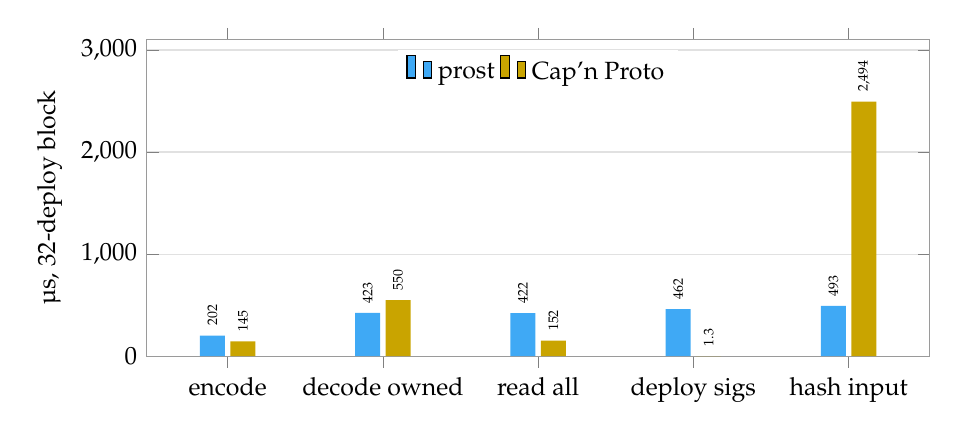
\begin{tikzpicture}
\begin{axis}[
  ybar, bar width=9pt, width=0.95\linewidth, height=5.6cm,
  ylabel={\si{\micro\second}, 32-deploy block}, ymin=0, ymax=3100,
  symbolic x coords={encode,decode owned,read all,deploy sigs,hash input},
  xtick=data, enlarge x limits=0.13,
  legend style={at={(0.5,0.97)},anchor=north,draw=none,font=\small,legend columns=-1},
  nodes near coords, every node near coord/.append style={font=\tiny,rotate=90,anchor=west},
  tick label style={font=\small}, label style={font=\small},
  axis line style={greyc}, ymajorgrids, grid style={greyc!30}]
\addplot[fill=protoc,draw=none] coordinates {(encode,202) (decode owned,423) (read all,422) (deploy sigs,462) (hash input,493)};
\addplot[fill=capnpc,draw=none] coordinates {(encode,145) (decode owned,550) (read all,152) (deploy sigs,1.3) (hash input,2494)};
\legend{prost,\capnp{}}
\end{axis}
\end{tikzpicture}
\caption{The 32-deploy, 40-events-per-deploy block. \capnp{} wins wherever the consumer can stay
on the reader; it loses wherever an owned structure or a canonical hash input is needed, which
is what the node's current architecture asks for.}
\label{fig:block}
\end{figure}

\begin{table}[h]
\centering\small
\begin{tabular}{@{}lrrrrrr@{}}
\toprule
& \multicolumn{2}{c}{prost} & \multicolumn{2}{c}{capnp} & \multicolumn{2}{c}{capnp packed} \\
\cmidrule(lr){2-3}\cmidrule(lr){4-5}\cmidrule(lr){6-7}
Workload & raw & +LZ4 & raw & +LZ4 & raw & +LZ4 \\
\midrule
block $32{\times}40$  & 206\,607 & 176\,846 & 294\,960 & 186\,953 & 234\,038 & 180\,209 \\
block $200{\times}40$ & 1\,281\,438 & 1\,093\,251 & 1\,820\,304 & 1\,154\,215 & 1\,449\,250 & 1\,112\,395 \\
\f{Par} medium & 4\,638 & 3\,379 & 32\,072 & 9\,962 & 13\,687 & 5\,942 \\
\f{Par} large & 28\,229 & 19\,438 & 188\,968 & 41\,896 & 81\,525 & 31\,421 \\
\bottomrule
\end{tabular}
\caption{Encoded sizes in bytes. Packed \capnp{} closes most of the gap but its encode
(268\,\si{\micro\second} on the 32-deploy block) and decode (661\,\si{\micro\second}) are then
slower than prost.}
\label{tab:sizes}
\end{table}

\subsection{Reading the numbers}

\begin{description}[style=nextline,leftmargin=0pt,font=\sffamily\bfseries\small]
\item[Encoding] \capnp{} building is 1.4--1.6$\times$ faster on blocks and 1.8--2.4$\times$
  faster on medium and large terms (slower on small ones). The term result is partly a prost
  artefact: protobuf length-prefixes every nested message and prost recomputes nested sizes at
  each level, so encode cost grows with depth$\times$size (28\,KB of \f{Par} costs more than twice
  as much to encode as a 207\,KB block).
\item[Owned decode] Building owned Rust values from a \capnp{} message costs more than prost's
  decode, because the reader still validates every pointer and the allocations are the same.
  Decoding prost from \f{Bytes} widens the gap: 278 vs.\ 550\,\si{\micro\second}.
\item[In-place reads] This is the \capnp{} advantage: a full walk is 3--5$\times$ cheaper than a
  prost decode, and selective access (deploy signatures) is three orders of magnitude cheaper. It
  is only available to code that consumes readers rather than owned structs.
\item[Hash inputs] \capnp{} admits many layouts for one value, so a hash needs
  \f{canonicalize()}: 3.6--7$\times$ the cost of prost encode for the same Blake2b. This rules
  \capnp{} out as the canonical \emph{hashing} format of a new shard release, even where it carries
  the wire and storage traffic (Sec.~\ref{sec:consensus}).
\item[Size] Unpacked messages are 43\% larger for blocks and nearly 7$\times$ larger for terms (8-byte
  alignment, pointer words, no varints). Every block is gossiped to every peer, so this is
  bandwidth, not just memory.
\end{description}

\section{The per-block budget}\label{sec:budget}

Table~\ref{tab:budget} traces a 32-deploy block through a receiving validator using the call
paths in the code and the timings above. Clones from \f{to_proto}/\f{from_proto} are estimated
by a struct clone of the same data.

\begin{table}[h]
\centering\small
\begin{tabular}{@{}L{7.2cm}L{5.0cm}r@{}}
\toprule
Step & Code & \si{\micro\second} \\
\midrule
Decode \f{BlockMessageProto} from \f{&[u8]} & \f{protocol/mod.rs:275} & 423 \\
\f{from_proto} into domain \f{BlockMessage} & \f{casper_message.rs} & $\approx$171 \\
Size metric: \f{to_proto} + full encode, length only & \f{block_processor.rs:542} & 373 \\
Hash check: \f{to_proto} + prost(header,body) + Blake2b & \f{validate.rs:1179} & 664 \\
Store: \f{to_proto} + encode + LZ4 & \f{key_value_block_store.rs:263} & 574 \\
\midrule
Total serialisation-related & & $\approx$\num{2200} \\
\quad of which prost encode/decode & & $\approx$\num{1030} \\
\bottomrule
\end{tabular}
\caption{Serialisation work per received 32-deploy block. For scale, the node's recorded propose
profile shows \f{checkpoint_compute_state} averaging 319\,ms (p95 460\,ms) and
\f{propose_total} 312\,ms (\f{docs/archive/adaptive-deploy-cap-validation-2026-03-05.md}).}
\label{tab:budget}
\end{table}

\noindent Protobuf encode/decode is therefore about 0.3\% of block handling, and everything
serialisation-related (including Blake2b and LZ4, which no codec choice removes) about 0.7\%.
A \capnp{} port that keeps the domain layer and a prost-style hashing encoding would change this
column as follows: decode $+127$; size metric $-373$ (the message knows its size); store encode $-228$; hash
check unchanged. Net saving $\approx$0.5\,ms per block, about 0.15\% of block time. A deeper port
that rewrites \f{casper} to consume readers directly (dropping \f{from_proto}) might reach
$\approx$0.8\,ms. The prost-side fixes in Section~\ref{sec:recs} recover $\approx$0.9\,ms with
a handful of line changes, and the Merkle-root hash of Section~\ref{sec:merkle} removes a further
$\approx$0.6\,ms from the end-of-block critical path.

\section{What a port would cost}

\begin{description}[style=nextline,leftmargin=0pt,font=\sffamily\bfseries\small]
\item[A new shard format] Because deployments adopt releases independently, a port can replace
  prost outright in a new format. The release must still define a canonical hashing encoding for
  the six families of Section~\ref{sec:consensus}, regenerate signed genesis contracts, and publish
  golden test vectors so that partner implementations agree byte-for-byte.
\item[The Rholang AST] capnp-rust generates readers and builders, not owned structs. The
  interpreter, normaliser, sorter, matcher and RSpace all operate on owned \f{rhoapi} values
  (with serde for bincode hashing, \f{Ord}, utoipa). Those structs stay; \capnp{} becomes one
  more conversion layer for the 58 term messages, hand-written or via a third-party derive.
\item[Client SDKs] Deploy signing happens in client code. Every SDK (pyf1r3fly, Embers,
  partner wallets such as ASI:Chain's) needs a signer for the new format, and must know which
  format a given shard speaks.
\item[Format identification] The handshake carries no protocol or format version; the only gate is
  \f{networkId} (\f{rp/connect.rs:450}). Nodes of one shard upgrade together, so no mixed-format
  shard is needed, but a format identifier in the handshake (and in the deploy API) would make a
  mismatched node or client fail with a clear error instead of a decode error.
\item[RPC and tooling] Cap'n Proto RPC is not gRPC. The Rust \f{capnp-rpc} crate is built around
  a single-threaded event loop (its examples run under Tokio's \f{LocalSet}/\f{spawn_local}),
  whereas \f{comm} is built on multi-threaded tonic with custom rustls interceptors, chunked
  streaming and circuit breakers. The practical route is a custom tonic \f{Codec} carrying
  \capnp{} bytes, which forfeits tonic-reflection and grpcurl for those services.
\item[External APIs] pyf1r3fly, system-integration and Embers use protobuf/gRPC stubs, and the
  HTTP API serialises the \f{rhoapi} types to JSON via serde. Moving the public API means new stubs
  for every client and partner integration; keeping it on protobuf means that surface gains nothing.
\item[Storage] New shards start with the new store format. A migrator is only needed for an
  existing deployment that wants to move its history rather than start a new shard; the
  \f{deploy_codec.rs} format tag shows the pattern.
\item[Size and safety] 43\% more bytes per gossiped block unless packed (which loses the speed);
  readers need traversal and nesting limits tuned against the 256\,MB stream ceiling.
\end{description}

\begin{table}[h]
\centering\small
\begin{tabular}{@{}L{6.0cm}L{6.6cm}r@{}}
\toprule
Scope & Main work & Eng.-weeks \\
\midrule
A.\ P2P payloads only (Casper + routing) & $\sim$70 messages to schema; conversions; tonic codec; format identifier in handshake & 5--8 \\
B.\ A + block/deploy storage & new store format; optional migrator for existing shards & +2--3 \\
C.\ B + hashing encoding redefined & canonical spec, golden vectors, SDK signers, genesis contracts & +2--3 \\
D.\ C + casper consuming readers directly & rewrite of block handling over 63+ files & +8--12 \\
E.\ Public APIs and \f{rhoapi} & client stubs, JSON layer, interpreter types & large; little gain \\
\bottomrule
\end{tabular}
\caption{Rough effort, assuming one engineer familiar with the code base. Ranges are judgement,
not measurement; the expected gain for A--D is under 0.3\% of block time
(Section~\ref{sec:budget}).}
\end{table}

\section{Using the freedom differently: a Merkle-root block hash}\label{sec:merkle}

Because hash formats are per-release, the block-hash input itself can be redesigned without any
change of codec. Today \f{hash_block} encodes the whole header and body and hashes them in one serial
pass at the end of validation, after cloning both through \f{to_proto}. The alternative hashes each
processed deploy on its own (a leaf), builds a binary Merkle tree over the leaves, and hashes the
header together with the root. A validator computes each leaf from its own replay result as that
deploy finishes, so at the end of the block only the tree and header remain.

\begin{table}[h]
\centering\small
\begin{tabular}{@{}lrrrr@{}}
\toprule
& \multicolumn{1}{c}{current} & \multicolumn{3}{c}{Merkle root over deploys} \\
\cmidrule(lr){2-2}\cmidrule(lr){3-5}
Workload & whole body & all leaves + root & root only & one leaf \\
\midrule
block $1{\times}40$   & 13.5 & 12.4 & 0.5 & 11.6 \\
block $32{\times}40$  & 463 & 468 & 7.0 & 11.7 \\
block $32{\times}400$ & 4\,733 & 4\,618 & 7.1 & 126 \\
block $200{\times}40$ & 3\,263 & 2\,918 & 43 & 13.6 \\
\bottomrule
\end{tabular}
\caption{Block-hash input cost in \si{\micro\second}, prost encoding plus Blake2b in both cases.
``root only'' is the end-of-block work when leaves were computed during replay.}
\label{tab:merkle}
\end{table}

\noindent The total hashing work is unchanged, but it moves off the critical path: for a 32-deploy
block the end-of-block check falls from 463 to 7\,\si{\micro\second}, and the \f{to_proto} clone
($\approx$171\,\si{\micro\second}) disappears, about 0.6\,ms in all. That is as much as the
\capnp{} port recovers, without touching the wire, storage or client APIs. The structure also brings
benefits a flat hash cannot:
\begin{itemize}
  \item a mismatching deploy is detected as soon as its replay finishes, not at the end of the
        block;
  \item leaves can be hashed in parallel across cores;
  \item any party can prove that a deploy and its result are in a block with $\lceil\log_2 n\rceil$
        sibling hashes, which matters to partner deployments that expose results to their own
        users or to light clients.
\end{itemize}
Deploy signatures, unforgeable seeds and the other families of Section~\ref{sec:consensus} are
unaffected and can stay on prost.

\section{Where \capnp{} would genuinely help}

The measured strengths are in-place and selective reads. Three places in the node could use them:
serving blocks to syncing peers straight from storage, look-ups that need a few fields of a stored
block (deploy signatures, parents), and very deep term encodes. The first two already have
cheaper answers within the current design: the block store has a bounded decoder and deploy-sig
cache (\f{key_value_block_store.rs:328-419}) and in-memory DAG caches, and stored bytes could be
forwarded to peers without a decode/re-encode. Deep term encodes happen off the hot path
(\f{toByteArray}, registry signatures, non-deterministic system-process outputs), and where they
matter for hashing, bincode already encodes them 6$\times$ faster than prost.

\clearpage
\section{Recommendations}\label{sec:recs}

\begin{enumerate}
  \item \textbf{Do not port.} Even with shard-format releases removing the need for a dual codec,
        the upper bound on the gain is a fraction of a percent of block time, against two to four
        months of engineering plus SDK and partner coordination.
  \item \textbf{Decode from \f{Bytes}.} \f{parse_packet} calls \f{T::decode(packet.content.as_ref())}
        (\f{casper/src/rust/protocol/mod.rs:275}); passing \f{packet.content.clone()} makes every
        \f{bytes} field a reference-counted slice. Measured: 35--40\% off block decode. Do the same
        for the block-store read path.
  \item \textbf{Stop encoding for a metric.} \f{block_processor.rs:542} runs \f{to_proto} and a
        full encode to record block size. Use the received byte length, or
        \f{encoded_len()} (14 vs.\ 202\,\si{\micro\second}).
  \item \textbf{Store what arrived.} For received blocks, the bytes on hand are already
        prost(\f{BlockMessageProto}); compress and store them instead of \f{to_proto}+encode. Keep
        re-encoding for locally created blocks.
  \item \textbf{Remove transport round trips.} The send path encodes a \f{Packet}, caches the
        bytes, decodes them, then chunks (\f{packet_ops.rs:89-109}); gossip de-duplication
        re-encodes each (small) gossip \f{Protocol} to hash it (\f{grpc_transport_receiver.rs:476}).
  \item \textbf{Move to a Merkle-root block hash in the next shard format}
        (Section~\ref{sec:merkle}). This removes the \f{to_proto} clone and the serial
        end-of-block encode, and adds per-deploy inclusion proofs. Until then, encode
        directly from the domain type (a hand-written \f{prost::Message::encode_raw}, pinned by
        golden tests) to drop the clone.
  \item \textbf{Measure the real hot path.} Add a criterion bench and a replay flamegraph for
        RSpace's bincode-plus-Blake2b channel hashing. That is where serialisation runs per
        produce/consume, and its bytes are part of the shard format too (\f{models/build.rs:93} already
        canonicalises \f{locally_free} for it).
  \item \textbf{Write down the canonical encoding, per shard format.} Shards currently depend on
        prost's behaviour (field order, \f{BTreeMap} maps, default-field elision). A short spec plus golden
        vectors, versioned with the shard format, protects deployments from a prost upgrade and
        lets partners implement compatible clients, whatever wire codec is chosen later.
\end{enumerate}

\section{Threats to validity}\label{sec:validity}

\begin{itemize}
  \item Workloads are synthetic. Event counts per deploy, term shapes and deploy sizes were chosen
        to be plausible, not sampled from a live shard. Exporting a few real blocks from a soak run
        and re-running the bench would remove this caveat.
  \item The node was not built or profiled, so the budget in Table~\ref{tab:budget} combines
        micro\-benchmarks with call-path reading; domain conversions are estimated by struct
        clones.
  \item A 2-vCPU shared VM; absolute numbers will differ on validator hardware, ratios less so.
  \item The \capnp{} \f{Par} schema covers the constructors the generator emits, not all 58
        \f{RhoTypes} messages; the full schema would not change the shape of the result.
\end{itemize}

\appendix
\section{Reproducing the benchmark}
The accompanying \f{serbench} crate contains \f{build.rs} (prost-build with the node's settings,
capnpc), \f{schema/f1r3.capnp}, copies of the two \f{.proto} files from \f{dev}, and
\f{src/main.rs}. It needs \f{protoc} and \f{capnp} on \f{PATH} and builds on stable Rust:
\begin{center}\texttt{cargo build -{}-release \&\& ./target/release/serbench}\end{center}
It writes \f{results.csv} (nanoseconds) and \f{sizes.csv}; the numbers in this note are from
those files.

\end{document}
